\documentclass[tikz]{standalone}
    \usetikzlibrary{arrows.meta, chains, calc, graphs, quotes, shapes.multipart}
    \begin{document}
    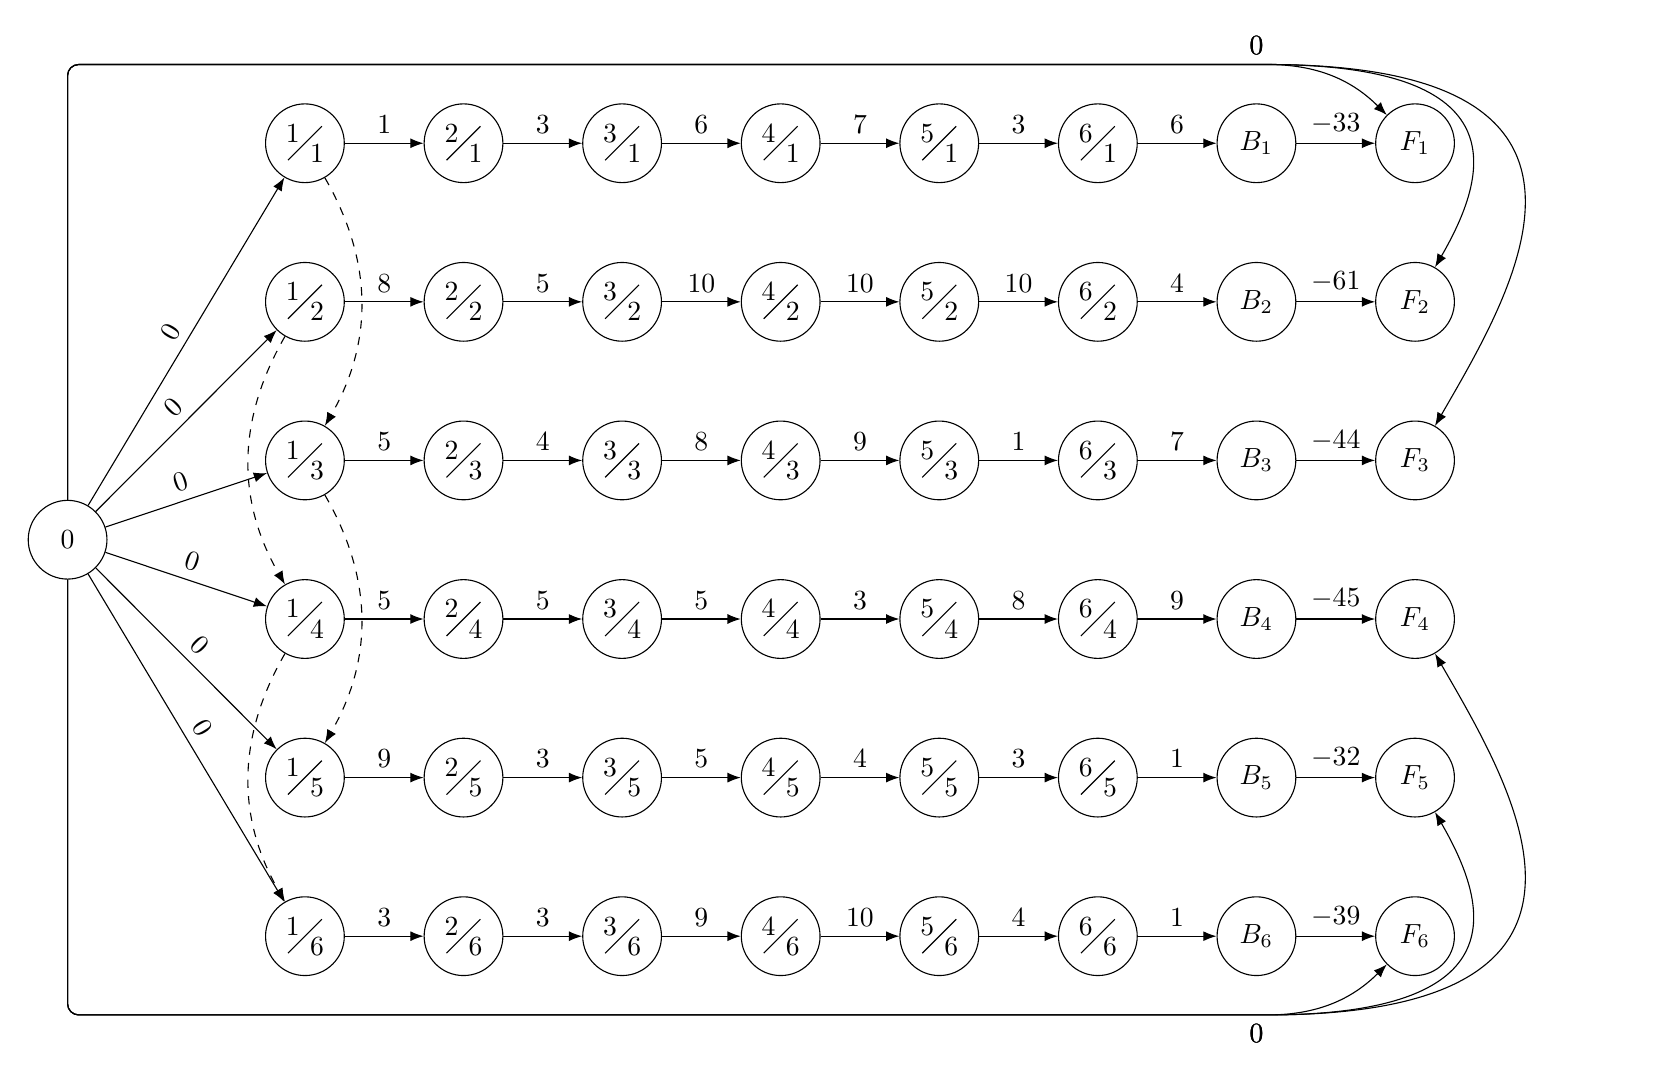
\begin{tikzpicture}[
      node distance=1cm,
      all nodes/.style={shape=circle, draw, minimum size=1cm},
      node BF/.style 2 args={
        all nodes, node other/.code=,shape=circle,
        name=#1 #2,node contents=$#1_{#2}$},
      node 7/.style={node BF={B}{#1}}, node 8/.style={node BF={F}{#1}},
      node other/.style 2 args={
        all nodes, shape=circle solidus, inner sep=.1em, name=#1 #2,
        node contents={#2 \nodepart{lower} #1}},
      >=Latex, every join/.style={->},
      start chain=rows going below,
    ]
    \foreach[count=\rowi] \rows in {{1, 3, 6, 7, 3, 6, -33},
                                    {8, 5, 10, 10, 10, 4, -61},
                                    {5, 4, 8, 9, 1, 7, -44},
                                    {5, 5, 5, 3, 8, 9, -45},
                                    {9, 3, 5, 4, 3, 1, -32},
                                    {3, 3, 9, 10, 4, 1, -39}}{
      \node[on chain, node other=\rowi 1];
      \tikzset{start branch={row\rowi} going right}
      \foreach[count=\coli from 2] \elem in \rows 
        \node[on chain, node \coli/.try=\rowi,
                        node other=\rowi\coli, join=by "$\elem$"];
    }
    \node[all nodes, left=2cm of $(3 1.west)!.5!(4 1.west)$](0){$0$}
      foreach \rowi in {1, ..., 6}{
        (0) edge[every join, "0" sloped] (\rowi\space 1)};
    
    \path[dashed] graph[edges=every join, use existing nodes]{
      1 1 ->[bend left]  3 1 ->[bend left]  5 1,
      2 1 ->[bend right] 4 1 ->[bend right] 6 1
    };
    \foreach \up/\Row/\above/\rows in {+/1/above/{1,2,3}, -/6/below/{6,5,4}}
      \foreach[count=\i from 0] \row in \rows
        \draw[rounded corners, every join] (0)
          |- node[at end, \above] {$0$} ([shift={(0,\up 1)}]B \Row.center)
          to[out=0, in/.evaluated={\up(\i==0?135:60)}, out looseness={1+1.5*sign(\i)}](F \row);
    \end{tikzpicture}
    \end{document}